One of the most critical design variables of the Hyperloop is the tube pressure
at which it operates. A lower pressure increases the power required of the
vacuum system in order to pump the tube down and maintain tube pressure for a
given leakage rate. However, it is known that the pressure at which the tube
operates will increase the density of the air and thus increase the power
requirements of both the electromagnetic propulsion system and the onboard compressor.
As compressor power demands change, the length and mass of the motor and
battery will change the pod geometry. Tube area is coupled with pod length,
as was shown in the boundary layer analysis, while the power required of the
electromagnetic propulsion system is coupled with pod mass. The boundary layer
that was described previously is used for this analysis. Tube pressure is
perhaps the single most important design variable to understand because it is
coupled with so many different aspects of system construction and performance.
Trade studies using this fully comprehensive system model can provide valuable
insight into the effects that variations in pressure have in every aspect of
design and performance at the system level.
Previous research has suggested that the ideal operating pressure should be on
the order of 100 Pa \cite{Musk, Chin}. However, such a low pressure could be
costly and difficult to implement across such a larger stretch of tube,
especially if there is significant leakage. It is likely that slight increases
in tube pressure could result in significant decreases in energy consumption
that could make up for increased drag penalty. To evaluate this, the full
system model will be run for a range of pressures. Tube area, compressor power,
steady state vacuum power, and total yearly energy consumption are recorded at each pressure.

\begin{figure}
	\centering
	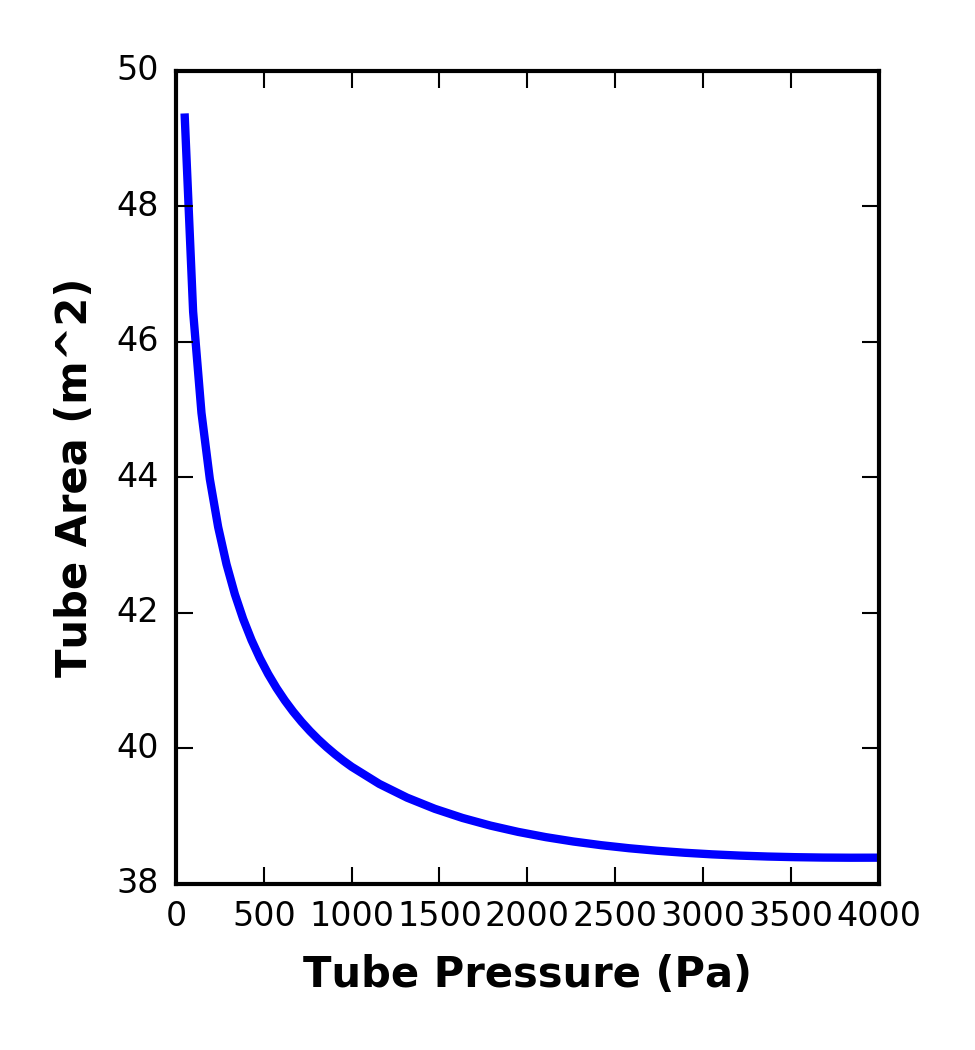
\includegraphics[width=.45\textwidth]{../../images/graphs/pressure_trades/pressure_vs_Area.png}
	\caption{Tube Area vs. Tube Pressure}
	\label{fig:tube_area_vs_tube_press}
\end{figure}
\Cref{fig:tube_area_vs_tube_press} shows tube area as a function of tube pressure.
As pressure increases, tube area decreases until leveling off around 3500 Pa.
This relationship is due to the effect that pressure has on boundary layer thickness.
Increasing the pressure increases the Reynolds number per unit length,
which decreases boundary layer thickness. As boundary layer thickness is
reduced the effective bypass area is increased which allows the tube area to
be reduced for the same Mach number. However, compressor power increases
linearly with pressure, which results in an increase pod length to hold a
larger motor and battery. As was shown previously, increasing length results in
increased boundary layer growth and causes tube size to grow. This trade
results in two-pressure regime, which are illustrated in \cref{fig:tube_area_vs_tube_press}.
At lower pressures, marginal increases in pressure result in decreases in tube
area because the increase in Reynolds number per unit length dominates the
length increases necessitated by higher compressor power demands. Meanwhile,
at higher pressures, increases in pod length begin to dominate boundary layer
sizing and the marginal effect on tube area is tempered.
\begin{figure}
	\centering
	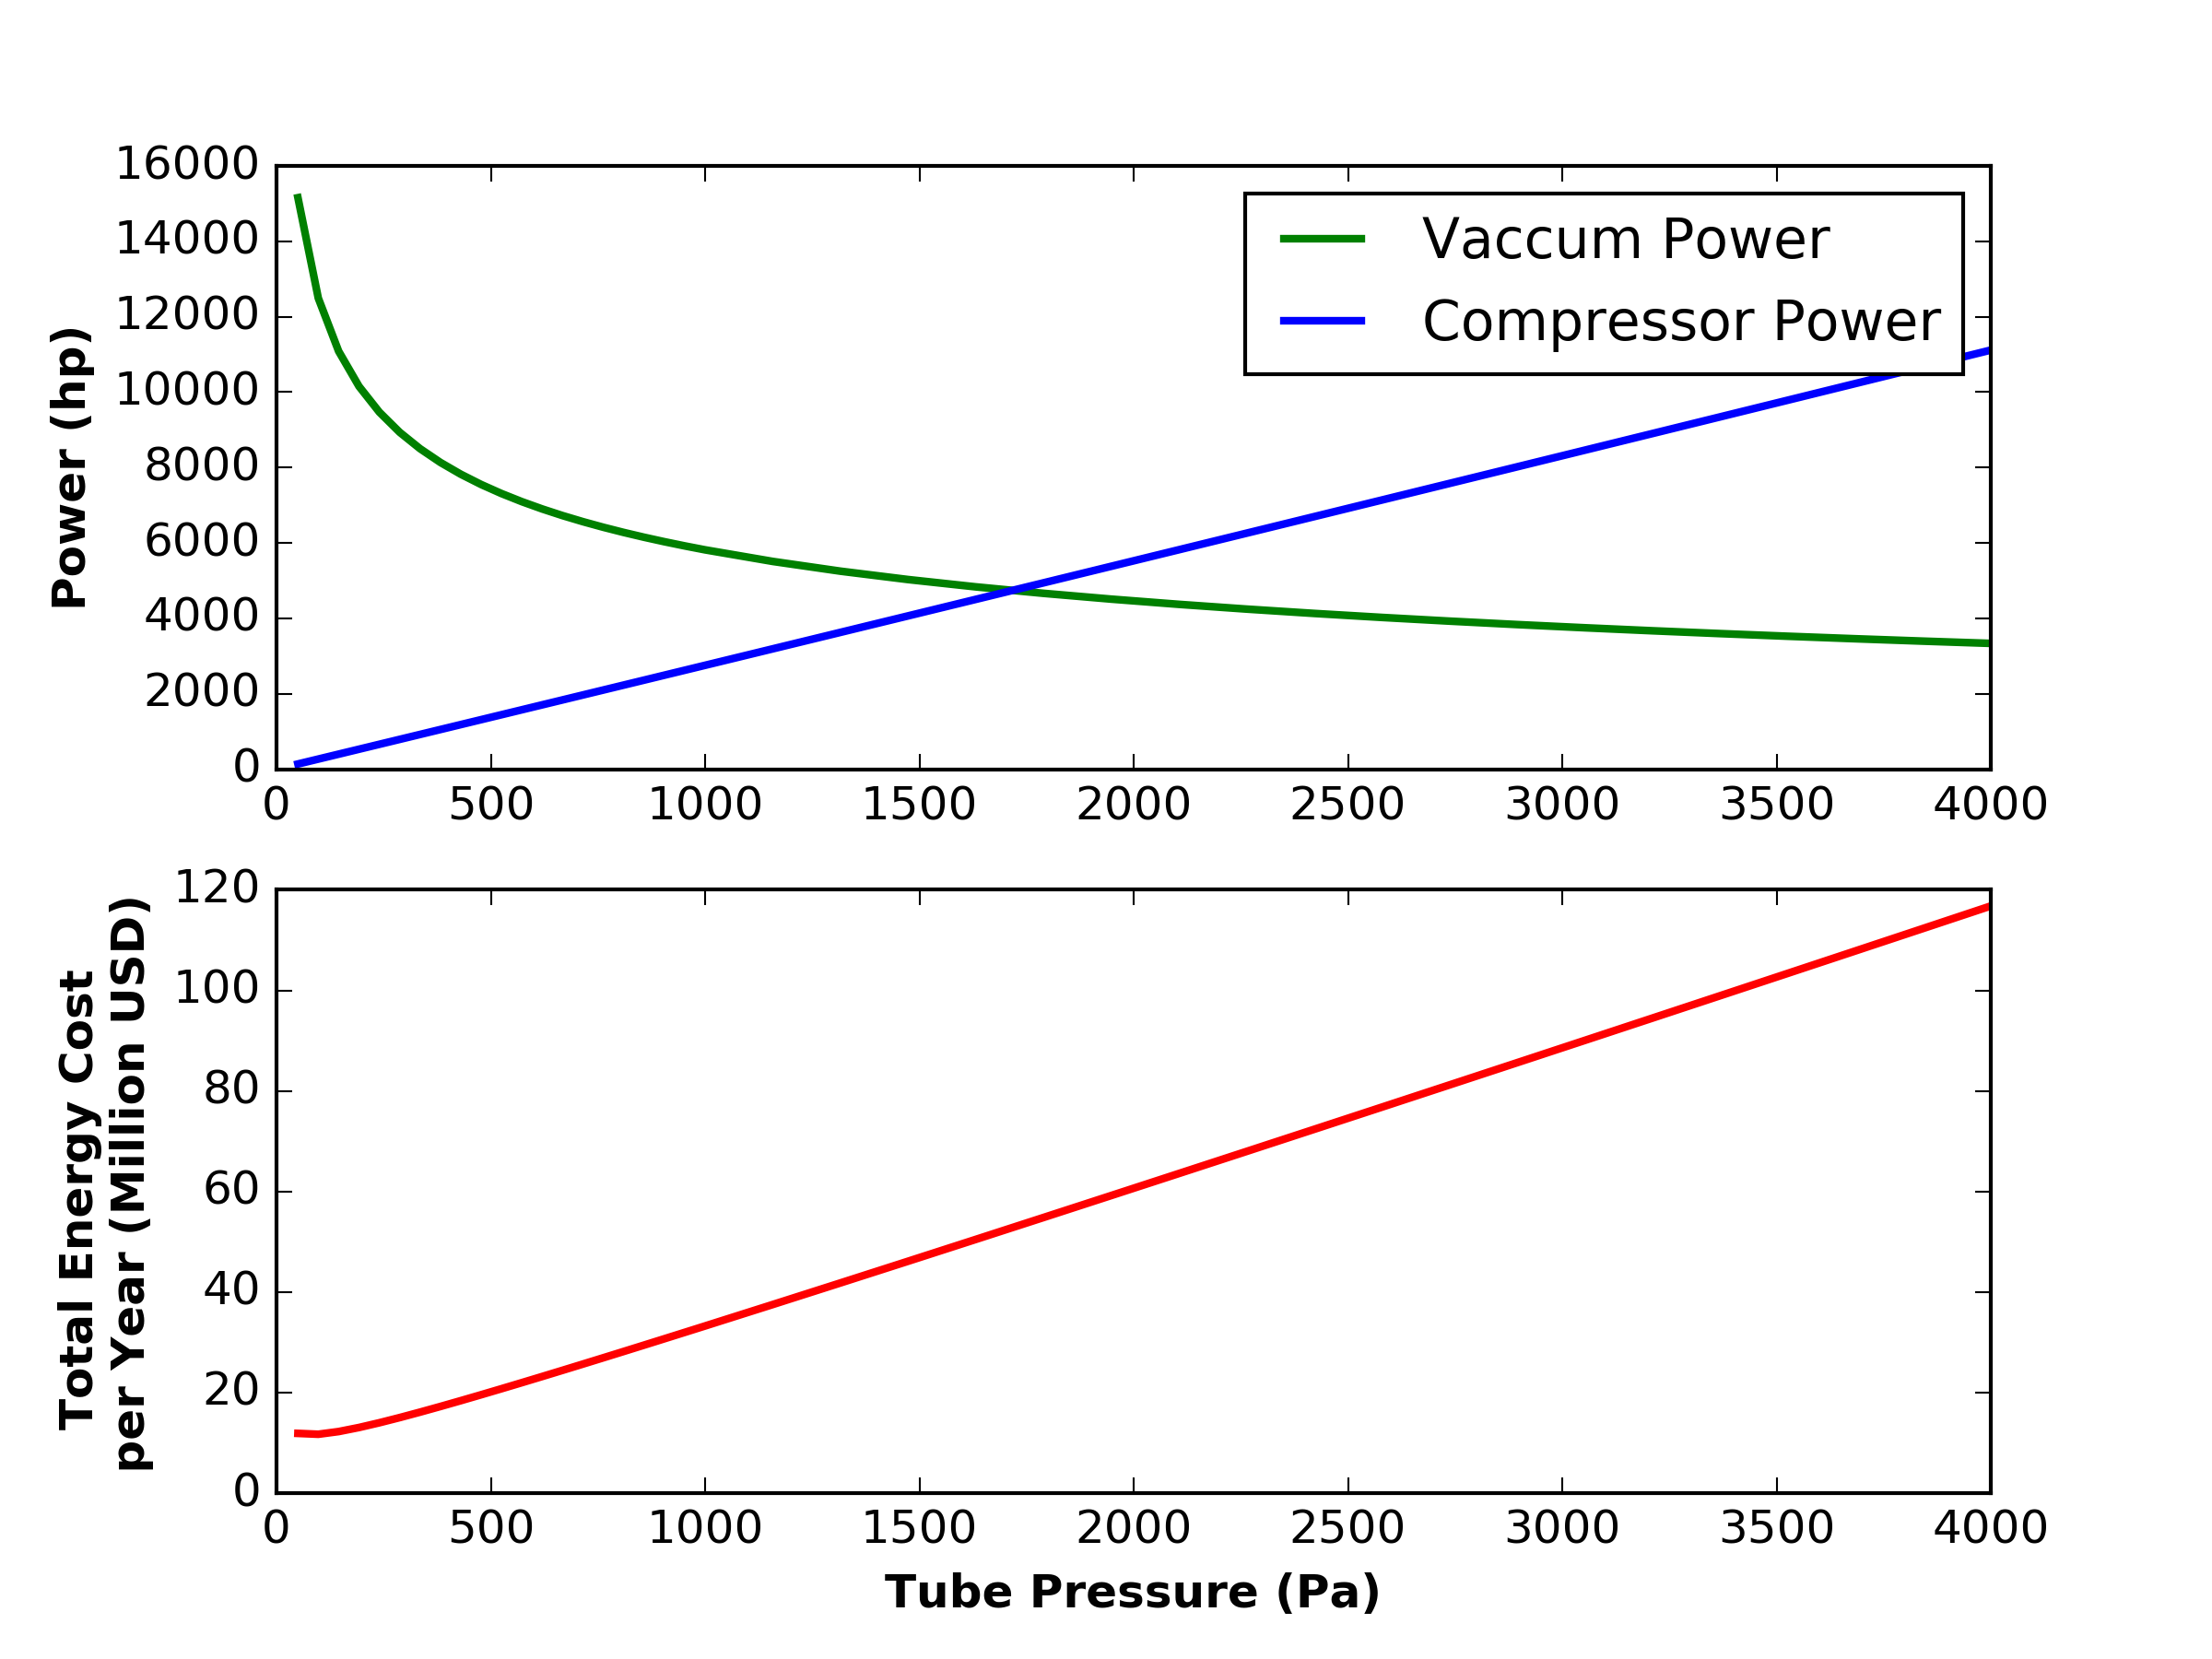
\includegraphics{../../images/graphs/pressure_trades/pressure_vs_power.png}
	\caption{Power Demands and Energy Consumption vs. Tube Pressure}
	\label{fig:pow_demands_vs_tube_press}
\end{figure}
\Cref{fig:pow_demands_vs_tube_press} shows how the power and energy consumption
change with tube pressure. As expected, high tube pressures require lower power
for a given leakage rate while requiring a higher power output from the onboard
compressor for a given compressor ratio. Thus, energy cost increases for very
low pressures due to the vacuum system and increases for very high pressures
due to increased power demand from the compressor.
The second plot in \cref{fig:pow_demands_vs_tube_press} shows that this
relationship produces a pressure at which energy cost is minimal. In this case,
the energy consumption is minimal at about 100 Pa. Energy consumption increases
fairly rapidly as pressure is increased beyond this minimum value. It is
important to note that this exact value is dependent on the leakage rate,
compressor pressure ratio, and whether or not regenerative braking is used to
recover battery energy (no regenerative braking is assumed in this analysis).
However, this relationship is crucial because it means that there does exist a
pressure that optimizes energy cost and that energy cost can increase rapidly
if deviations from this optimum point exist. A higher fidelity model can be
used to determine exactly what value of pressure optimizes energy consumption
for a given configuration. A more detailed examination of the effects that
leakage has on optimum pressure will be conducted next.
